\chapter{Environment}
This section will explain how to set up and start a bot with the starcraft environment using the GOAL programming language.

\section{Chaoslauncher}
In order to make use of all the starcraft brood war plugin, you can make use of the application: the chaoslauncher. With this application several plugins can be used like the: \textit{BWAPI Injector} which is neccesary for using the BWAPI library. It is also recommended to make use of the plugin: \textit{APMAlert}, which shows the current actions per minute of all your units together. When the APM of your bot is suddenly very high, your agents might be using to many actions in a row. At last it is also recommonded to make use of the \textit{W-Mode} plugin. This plugin automatically sets your Starcraft game in windowed mode which makes it easier for debugging. 

\section{Installation}
\begin{itemize}
    \item Download the starcraft environment MSI installer. After running the installer you can find in the installation folder the environment jar and a folder with 3 examples bots (one for each race).
    \item You can import one of the Example bots in your eclipse IDE. In the mas2g are some specified values, this will be discussed in \ref{mas2g}, but for now you can run the bot for testing purposes.
    \item After running the bot, the chaoslauncher should be automatically launched. If this is not the case please read \ref{mas2g}. When running the chaoslauncher, please check the BWAPI Injector (and W-Mode for your own convenience) if this is not already done. From here you should be able to click on start which will launch the game. The running GOAL bot will automatically connect to the game and start controlling your units. If the game does not start immediately, it could be generating the map data. If so please wait up to 2 minutes before doing anything, generating the map data only has to happen once for each map you want to use.
\end{itemize}

\section{The Mas2g}
\label{mas2g}
The starcraft environment offers multiple parameters to be set up in the mas2g. Within the mas2g you can specify which map you want to play, specify your own race, give up the map location of your starcraft game, turn the development tool on or off, enable the automenu script and specify which race you want to play against.

\begin{verbatim}
    use StarcraftEnvironment.jar as environment with
        map="(2)Destination.scx",
        own_race="terran",
        starcraft_location="C:\\Starcraft",
        debug="true",
        auto_menu="Single_Player",
        enemy_race="zerg".
\end{verbatim}

\subsection{Map}
\label{map}
It is possible to specify which map the chaoslauncher will automatically load when starting the game. This can be done by inserting the following line: \textit{map = <filename>}, where \textit{<filename>} is the exact filename of the map (with extension). Please note that the environment will only choose maps in the directory: \textit{Starcraft/maps/sscai/}. The installer provides the \textit{mapData} of 1 map, however you can use as many maps as you want. When choosing an other map in the \textit{sscai} folder please note that the first time running the environment will take some time (around 2 minutes) to generate the data of the given map. This only has to happen once, so it won't have to generate more than once.

\subsection{Own Race}
\label{own race}
You may also specify the race of your bot in the mas2g. This will automatically launch the chaoslauncher with the specified race. You can do this by inserting the following line: \textit{own\_race = <RaceName>}, where \textit{<RaceName>} can either be \textit{zerg}, \textit{protoss}, \textit{terran} or \textit{random}. The option \textit{random} will choose one race with 1/3 of a chance for each race. 

\subsection{Starcraft\_Location}
\label{starcraft location}
It is also possible to specify the location of the source map of the starcraft game. When using the starcraft game provided by the environment installer, this feature will automatically start the chaoslauncher when launching the GOAL bot. When the chaoslauncher is already running it won't start again untill you close it. When the Choaslauncher is automatically started by the environment, an automatic script will be written with all the necessary information to run the GOAL bot (so it is recommended to use this feature). You can use this feature by inserting the line: \textit{starcraft\_location = <FilePath>}, where \textit{<FilePath>} is the absolute path to the starcraft source folder.

\subsection{Debug}
\label{debug}
The Environment also offers a development tool for debugging purposes. With this development tool you can increase or decrease the game speed, enable cheats and draw unit and map details on screen. More information about the development tool can be found at \ref{development tool}. For using the development tool you can insert the following line: \textit{debug=<Boolean>}, where \textit{<Boolean>} will indicate for enabling or disabling the development tool.

\subsection{Auto Menu}
\label{auto menu}
The auto menu parameter can be used to quickly go through the menu of the game when starting your agent. This can be used for single player games and multi player games. For using the auto menu function you can insert the following line: \textit{auto\_menu=<MenuChoice>}, where \textit{<MenuChoice>} is either \textit{Single\_Player} for a single player game or \textit{Multi\_Player} for a multi player game.

\subsection{Enemy Race}
\label{enemy race}
The enemy race parameter can be used for specifying which race you want to play against. When an actual enemy race is chosen like: \textit{zerg}, \textit{protoss} or \textit{terran} the \textit{enemyRace} percept will indicate against which race you are playing, while when not specifying an enemy race, so when the option: \textit{random} is chosen, the \textit{enemyRace} percept will be \textit{Unknown} untill the opponent is scouted for the first time. For using the enemy race parameter you can insert the following line: \textit{enemy\_race=<RaceName>}, where \textit{<RaceName>} can either be \textit{zerg}, \textit{protoss}, \textit{terran} or \textit{random}. The option \textit{random} will choose one race with 1/3 of a chance for each race. 

\subsection{Defining an agent}
When defining an agent it is important that the right type is given to the agent. This has to be the same type of the starcraft unit where the first letter is non-capital. So for example when you want to add a terran SCV agent, this can be done by defining the type of this agent as: \textit{terranSCV}. Note that each unit type first begins with the race of the unit and is followed by the exact name of the unit type.

\begin{verbatim}
    define myAgent as agent {  
        use MyAgentInit as init module.
        use MyAgent as main module.
        use MyAgentEvent as event module.
    }
    
    launchpolicy {
        when type = terranSCV launch myAgent.
    }
\end{verbatim}


\newpage
\section{The Development Tool}
\label{development tool}

\begin{figure}[h]
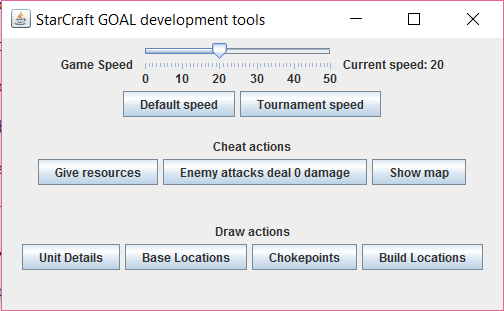
\includegraphics[width=1.0\textwidth]{images/developmentTool}
\caption{Example of the Development Tool}
\label{fig:starcraft_picture}
\end{figure}

\subsection{Game Speed}
The Game Speed slider can be found at the top of the development tool window. This can be used to quickly change the speed of the game. The initial game speed is set to 20. The fastest game speed is 50 and the slowest game speed is 0. Please note that the agent is supposed to play normally at game speed 30 which is the default game speed for AI tournaments. When the speed is set to 50, the agents can react slower than they would be on the tournament gamespeed. Setting the game speed on 50 should only be used for quick testing purposes.

\subsection{Cheat Actions}
The development tool offers 3 buttons which instantly enable cheats. Note that these cheats should be used for testing purposes only. The first cheat is called: \textit{Give resources} which gives the player 10000 minerals and 10000 gas. The second cheat is called: \textit{Enemy attacks deal 0 damager} which makes the units of the player immune for damage. The last cheat is called: \textit{Show map} which makes the whole map visible for the player. Note that also all your agents will be perceiving everything on the map. 

\subsection{Map drawing}
The development tool can also be used to show map or unit details. There are 4 buttons which can be used. First there is the \textit{Unit Details} button which shows the health and \textit{ID} of every unit. There is also the \textit{Base Locations} button which shows all the starting locations of the map and also all the base locations on the map where players could be expanding to. There is also the \textit{Chokepoints} button which shows all the chokepoints (which are the narrow points where not many units can go through at the same time) on the map. At last there is the \textit{Build Locations} button which shows all the non-obstructed and explored building locations of the map which the worker units perceive with the \textit{constructionSite} percept. 

